\documentclass[../main.tex]{subfiles}
\graphicspath{{\subfix{../figures/}}}

\begin{document}

\chapter{{DiffFracQuant: A Bayesian Model for the Detection of Differential Fractionation}}

\section{Chapter 5 Introduction}

Localisation of RNA populations to specific sub-cellular compartments is a widely implemented mechanism to regulate gene expression.
Focusing localisation machinery on mRNA transcripts rather than proteins is more energy efficient as one mRNA transcript can lead to the translation of hundreds of proteins \parencite{Chin2017}.
Rapid changes in gene expression in response to stimuli such as heat stress can be achieved by chaperoning surplus mRNA transcripts into stress granules where translation may be supressed \parencite{Anderson2009}.
In plant and animal cells, microRNA (miRNA), long non-coding RNA (lncRNA) and small interfering RNA (siRNA) contribute to gene expression regulation through splicing, degradation or translation pathways specific either to the nucleus or cytoplasm \parencite{Hombach2016}.

Several RNA-Seq assays have been developed to isolate and compare RNA populations in different sub-cellular compartments.
Fractions of mRNA from organelles of different weights can be separated by centrifuging lysed cells. 
Centrifuging using a sucrose gradient or by repeating the process on the supernatent under increasing speeds can separate multiple fractions within an experiment \parencite{Iserman2020, Dunham2012, Hu2017}.
Alternatively, fractions of freely floating vs protein bound mRNA can be separated by orthogonal organic phase separation \parencite{Queiroz2019}. 
Despite the development of multiple fractionation-based RNA-Seq assays, there are a limited number of statistical methods to analyse them.

RNASeq datasets need to be normalised to remove batch effects and flow cell dependent biases often introduced during reverse transcription and amplification. 
Differential expression analysis is easily confounded by RNA-Seq biases if they are not removed \parencite{Soneson2018}.
For example, the amplification of reads from each lane of a RNA-seq machine can vary significantly. 
The shotgun method of short read sequencing also introduces a length bias the number of reads per gene will be proportional to the length of that gene. 
In addition elongation biases between the nucleotides can change the amplification ratio of genes.
Certain gene with high GC content may not be amplified as efficiently because the complimentary bases bind too tightly for the melting stage to occur. 
These sequences biases mean raw reads are rarely used as the measure of expression between samples and between genes. 

Sequencing biases can be removed by normalising to internal or external controls. 
Internal normalisation commonly consists of converting raw reads into transcripts per million (TPM).
Previously, fragments per kilobase million (FPKM) was used as a normalised read counts, but it was found to ohave unwanted properties \parencite{Wagner2012}.
Transcripts per million account for the total read variation between runs and the gene length biases. 
However, dividing by the total number of reads in a run does introduce a dependence on the behaviour of a few highly expressed genes.
The large order of magnitude difference in expression across an organisms genome leads to genes that are expressed on the order of $10^4$ transcripts per cell contributing more to the total reads compared to transcripts that only occur once or twice. 
If the experiments significant change the expression of the highly expressing genes comparing TPM may confound expression patterns. 
Alternatively, an external control of known volumes of synthetic RNA can be introduced with differing GC content and lengths. 
The comparison of these RNA levels after being amplified in the RNA-seq assay can discover biases in transcript length, total read and GC content \parencite{Evans2018}.
However, errors in the volumes of spike-in RNAs added to each run can significantly impede the effectiveness of the method.

An alternative internal control is based on quantile normalisation.
Techniques such as the median of medians used by DESeq2 attempts to find the behaviour of the average gene across the condition \parencite{Anders2010}.
Under the assumption that most genes do not express differently across genes the change in the most average gene must be down to sequencing biases.
This assumption breaks down in cases where the majority of gene are expected to have different expression across RNA-Seq samples. 
DESeq2 also uses shrinkage methods to reduce variance in lowly expressed genes \parencite{Love2014}.
However, the method in DESeq2 assumes the majority of genes are expressed at similar levels across conditions. 
It uses this assumption to share dispersion information across genes so that gene-wise shrinkage estimates can be determined to account for biases. 
In assays that extract RNA from different fractions, changes in abundance across the entire transcriptome can be expected invalidating DESeq2’s assumptions.


The work here outlines an alternative way of normalising RNA-Seq data sets that compare fractions using the additional information that can be gathered when measure subsets of a complete cell.
This will enable even more sensitive comparisons of transcript localisation across conditions and cell types.
DiffFracQuant is an open source R package that detects differences in transcript fractionation using a Bayesian hierarchical model.

\section{Chapter 5 Results}

\subsection{Bayesian Hierarchical Model}

The fundamental basis of the DiffFracQuant's model for detecting differential fractionation is that for any particular gene the sum of transcripts counts from sub-fractions must equal the counts from the total body; i.e. $N^{Tot} = N^{A}+N^{B}$.
Therefore, the information gained from sequencing a sample before fractionation can be used remove the noise associated with RNA-Seq data and enable accurate comparison of fractions.
The noise of transcript counts from RNA-Seq data is modeled by a negative binomial with mean $\lambda$ and overdispersion parameter $\phi$.
The DiffFracQuant model contains three negative binomial distributions: one for samples from the total body and one for each of the two sub-fractions Figure \ref{fig:DiffFracQuant-plate-diagram}.
The three negative binomial distributions each have a overdispersion parameter: $\phi^{Tot}$, $\phi^{A}$ and $\phi^{B}$, that is shared across genes and conditions.
Separate mean parameters for transcript counts are learnt for the sub-fraction negative binomials: $\lambda^A$ and $\lambda^B$, and their sum is used as the mean for the total negative binomial.
The $\lambda$ parameters are determined in log space to help the model to fit the broad range of transcript count levels expected across an entire genome.
In addition to the mean transcipt count parameter, each negative binomial has a total reads scale factor term: $a^{Tot}$, $a^{A}$, $a^{B}$, that is unique to the condition and replicate used.
The R package RStan is used to sample from the posterior distribution.

\begin{figure} [t!]
     \centering
     \begin{subfigure}[b]{0.54\textwidth}
     \centering
     \tikz{
        % Nodes
        \node[obs]                                   (N-t)   {$N^{Tot}_{grc}$}; %
        \node[obs, above=1 of N-t, xshift=-1.2cm]     (N-s)   {$N^{A}_{grc}$}; %
        \node[obs, right=1 of N-s, xshift=0.4cm]     (N-p)   {$N^{B}_{grc}$}; %
        \node[latent, above=1 of N-s]  (l-s)   {$\lambda^{A}_{gc}$}; %
        \node[latent, above=1 of N-p] (l-p)   {$\lambda^{B}_{gc}$}; %
        \node[latent, left=2 of N-t, xshift=-1cm] (p-t)     {$\phi^{Tot}$}; %
        \node[latent, above=1 of p-t] (p-s)     {$\phi^{A}$}; %
        \node[latent, right=1 of N-p, xshift=0.4cm] (p-p)     {$\phi^{B}$}; %
        \node[latent, below=1 of N-t] (a-t)     {$a^{Tot}_{cr}$}; %
        \node[latent, left=1 of a-t, xshift=-0.3cm] (a-s)     {$a^{A}_{cr}$}; %
        \node[latent, right=1 of a-t, xshift=0.2cm] (a-p)     {$a^{B}_{cr}$}; %
        \node[latent, below=3 of N-t, yshift=-0.4cm] (alpha-p)     {$\alpha$}; %
        \node[latent, above=4 of N-t, yshift=0.5cm] (sigma)     {$\sigma^2$}; %
        \node[latent, above=1 of sigma, yshift=-0.5cm] (mu)     {$\mu$}; %
        
        
        % Connections
        \edge {a-t} {N-t} ; %
        \edge {a-s} {N-s} ; %
        \edge {a-p} {N-p} ; %
        \edge {p-t} {N-t} ; %
        \edge {p-s} {N-s} ; %
        \edge {p-p} {N-p} ; %
        \edge {l-s} {N-t, N-s} ; %
        \edge {l-p} {N-t, N-p} ; %
        \edge {alpha-p} {a-p, a-s} ; %
        \edge {sigma} {l-s, l-p} ; %
        \edge {mu} {l-s, l-p} ; %
        
        % plate
        \plate {rep} {(N-t)(N-p)(N-s)(a-t)(a-p)(a-s)} {$Rep$}
        \plate {gene} {(l-p)(l-s)(N-t)(N-p)(N-s)} {$Gene$}
        \plate {con} {(N-t)(N-p)(N-s)(gene)(rep)} {$Con$}
    }
    \end{subfigure}
     \hfill
     \begin{subfigure}[b]{0.44\textwidth}
     \centering
     \begin{align*}
        N^{Tot}_{grc} & \sim  negbin(a^{Tot}_{cr}(e^{\lambda^{A}_{gc}} + e^{\lambda^{B}_{gc}}), \phi^{Tot})\\
        N^{B}_{grc} & \sim  log\_negbin(a^{B}_{cr}+\lambda^{B}_{gc}, \phi^{B})\\
        N^{A}_{grc} & \sim  log\_negbin(a^{A}_{cr}+\lambda^{A}_{gc}, \phi^{A})\\
     \end{align*}
     \begin{align*}
        \lambda^{A}_{gc}, \lambda^{B}_{gc} &\sim normal(\mu, \sigma^2)\\
        \mu &\sim normal(7,2)\\
        \sigma^2&\sim normal(2,1)\\
        \phi^{Tot}, \phi^{A}, \phi^{B}&\sim normal(100,10)\\
        a^{Tot}_{cr}&\sim normal(10, 0.1)\\
        a^{A}_{cr}, a^{B}_{cr}&\sim normal(\alpha, 0.1)\\
        \alpha&\sim normal(0, 0.5)
    \end{align*}
    \vspace{0.5cm}
     \end{subfigure}
     \caption[Overview of DiffFracQuant Model.]{\textbf{Plate diagram summarising the Bayesian hierarchical model behind DiffFracQuant.} Shaded circles represent observed variables, in this case the unnormalised RNA-Seq transcript counts, and white circles represent latent variables learnt by the model. Circles placed within a square plate have separate random variables for each possible value associated with that plate, i.e. the $a^{A}$ circle is within the Rep plate and Con plate as there is a $a^{A}$ for each replicate and condition.}
     \label{fig:DiffFracQuant-plate-diagram}
\end{figure}

\subsection{Test Data Sets}
The performance of DiffFracQuant compared to DESeq2 is tested using three data sets: two experimental and one simulated.
The simulated data set consists of 300 genes with total transcript counts, $X^{Tot}$, sampled from a lognormal distribution to simulate the range of gene expressions in an RNA-Seq data set.
The ratio of transcripts between fraction A and B for each gene, $\gamma$, is sampled from a beta distribution to give a range of effect sizes.
The parameters of the beta distribution were set to simulate three regimes: all gene are randomly allocated a fraction, most genes have a marginal bias towards fraction A, and the majority of transcripts are in fraction A but transcripts from a specific subset of genes are found in fraction V, Figure \ref{fig:fractionation-datasets}A.
Noise typically associated with RNA-Seq data sets is introduced to the ideal genewise transcript counts by sampling from a negative binomial with mean equal to the ideal value creating the training data, $N^{A}$, $N^{B}$ and $N^{Tot}$.
Three data points are sampled for each gene in each fraction and condition to create three replicates.
Finally, a RNA-Seq run specific parameter, $\alpha$, is introduced to represent the varying total reads expected from every replicate, condition and fraction sequencing run.

$$X^{Tot}_g \sim lognormal(\mu, \sigma^2)$$
$$N^{A}_{grc} \sim negbin(\gamma_{gc}\alpha^{A}_{rc}X^{Tot}_g,\phi)$$
$$N^{B}_{grc} \sim negbin((1-\gamma_{gc})\alpha^{B}_{rc}X^{Tot}_g,\phi)$$
$$N^{Tot}_{grc} \sim negbin(\alpha^{Tot}_{rc}X^{Tot}_g,\phi)$$
$$\alpha \sim uniform(min=0.5, max=3)$$
$$\gamma_{gc}\sim beta(a_c,b_c)$$

The first experimental data set comes from the Encyclopedia of DNA Elements (ENCODE) consortium \parencite{Dunham2012}. 
It was downloaded from the ENCODE portal with the following identifiers: ENCSR000COR, ENCSR000COQ, ENCSR000CPO.
The data set consists of total, nuclear and cytoplasmic poly(A) RNA transcripts from a human GM12878 lymphoblastoid cell line.
The fractions were separated using centrifugation and include two bioreps, Figure \ref{fig:fractionation-datasets}B.
The reads were already aligned to the hg38 human reference genome and counted by the RSEM software following the standard ENCODE analysis pipeline \parencite{Luo2020}.
The second experimental data set is from a paper investigating the formation of heat-induced stress granules in \textit{Saccharomyces} cerevisiae.
RNA transcripts held in stress granules were pelleted by 18,000g centrifugation and are available alongside transcripts freely floating in the supernatant and transcripts sampled before centrifugation across two bioreps, Figure \ref{fig:fractionation-datasets}C.
The reads were already aligned to the S288C reference genome (release R64-2-1) and counted used the STAR aligner.
The \textit{Saccharomyces} data set also includes a deletion strain in each of the three temperatures, but it is not used here. 

\begin{figure}[p!]

{\centering 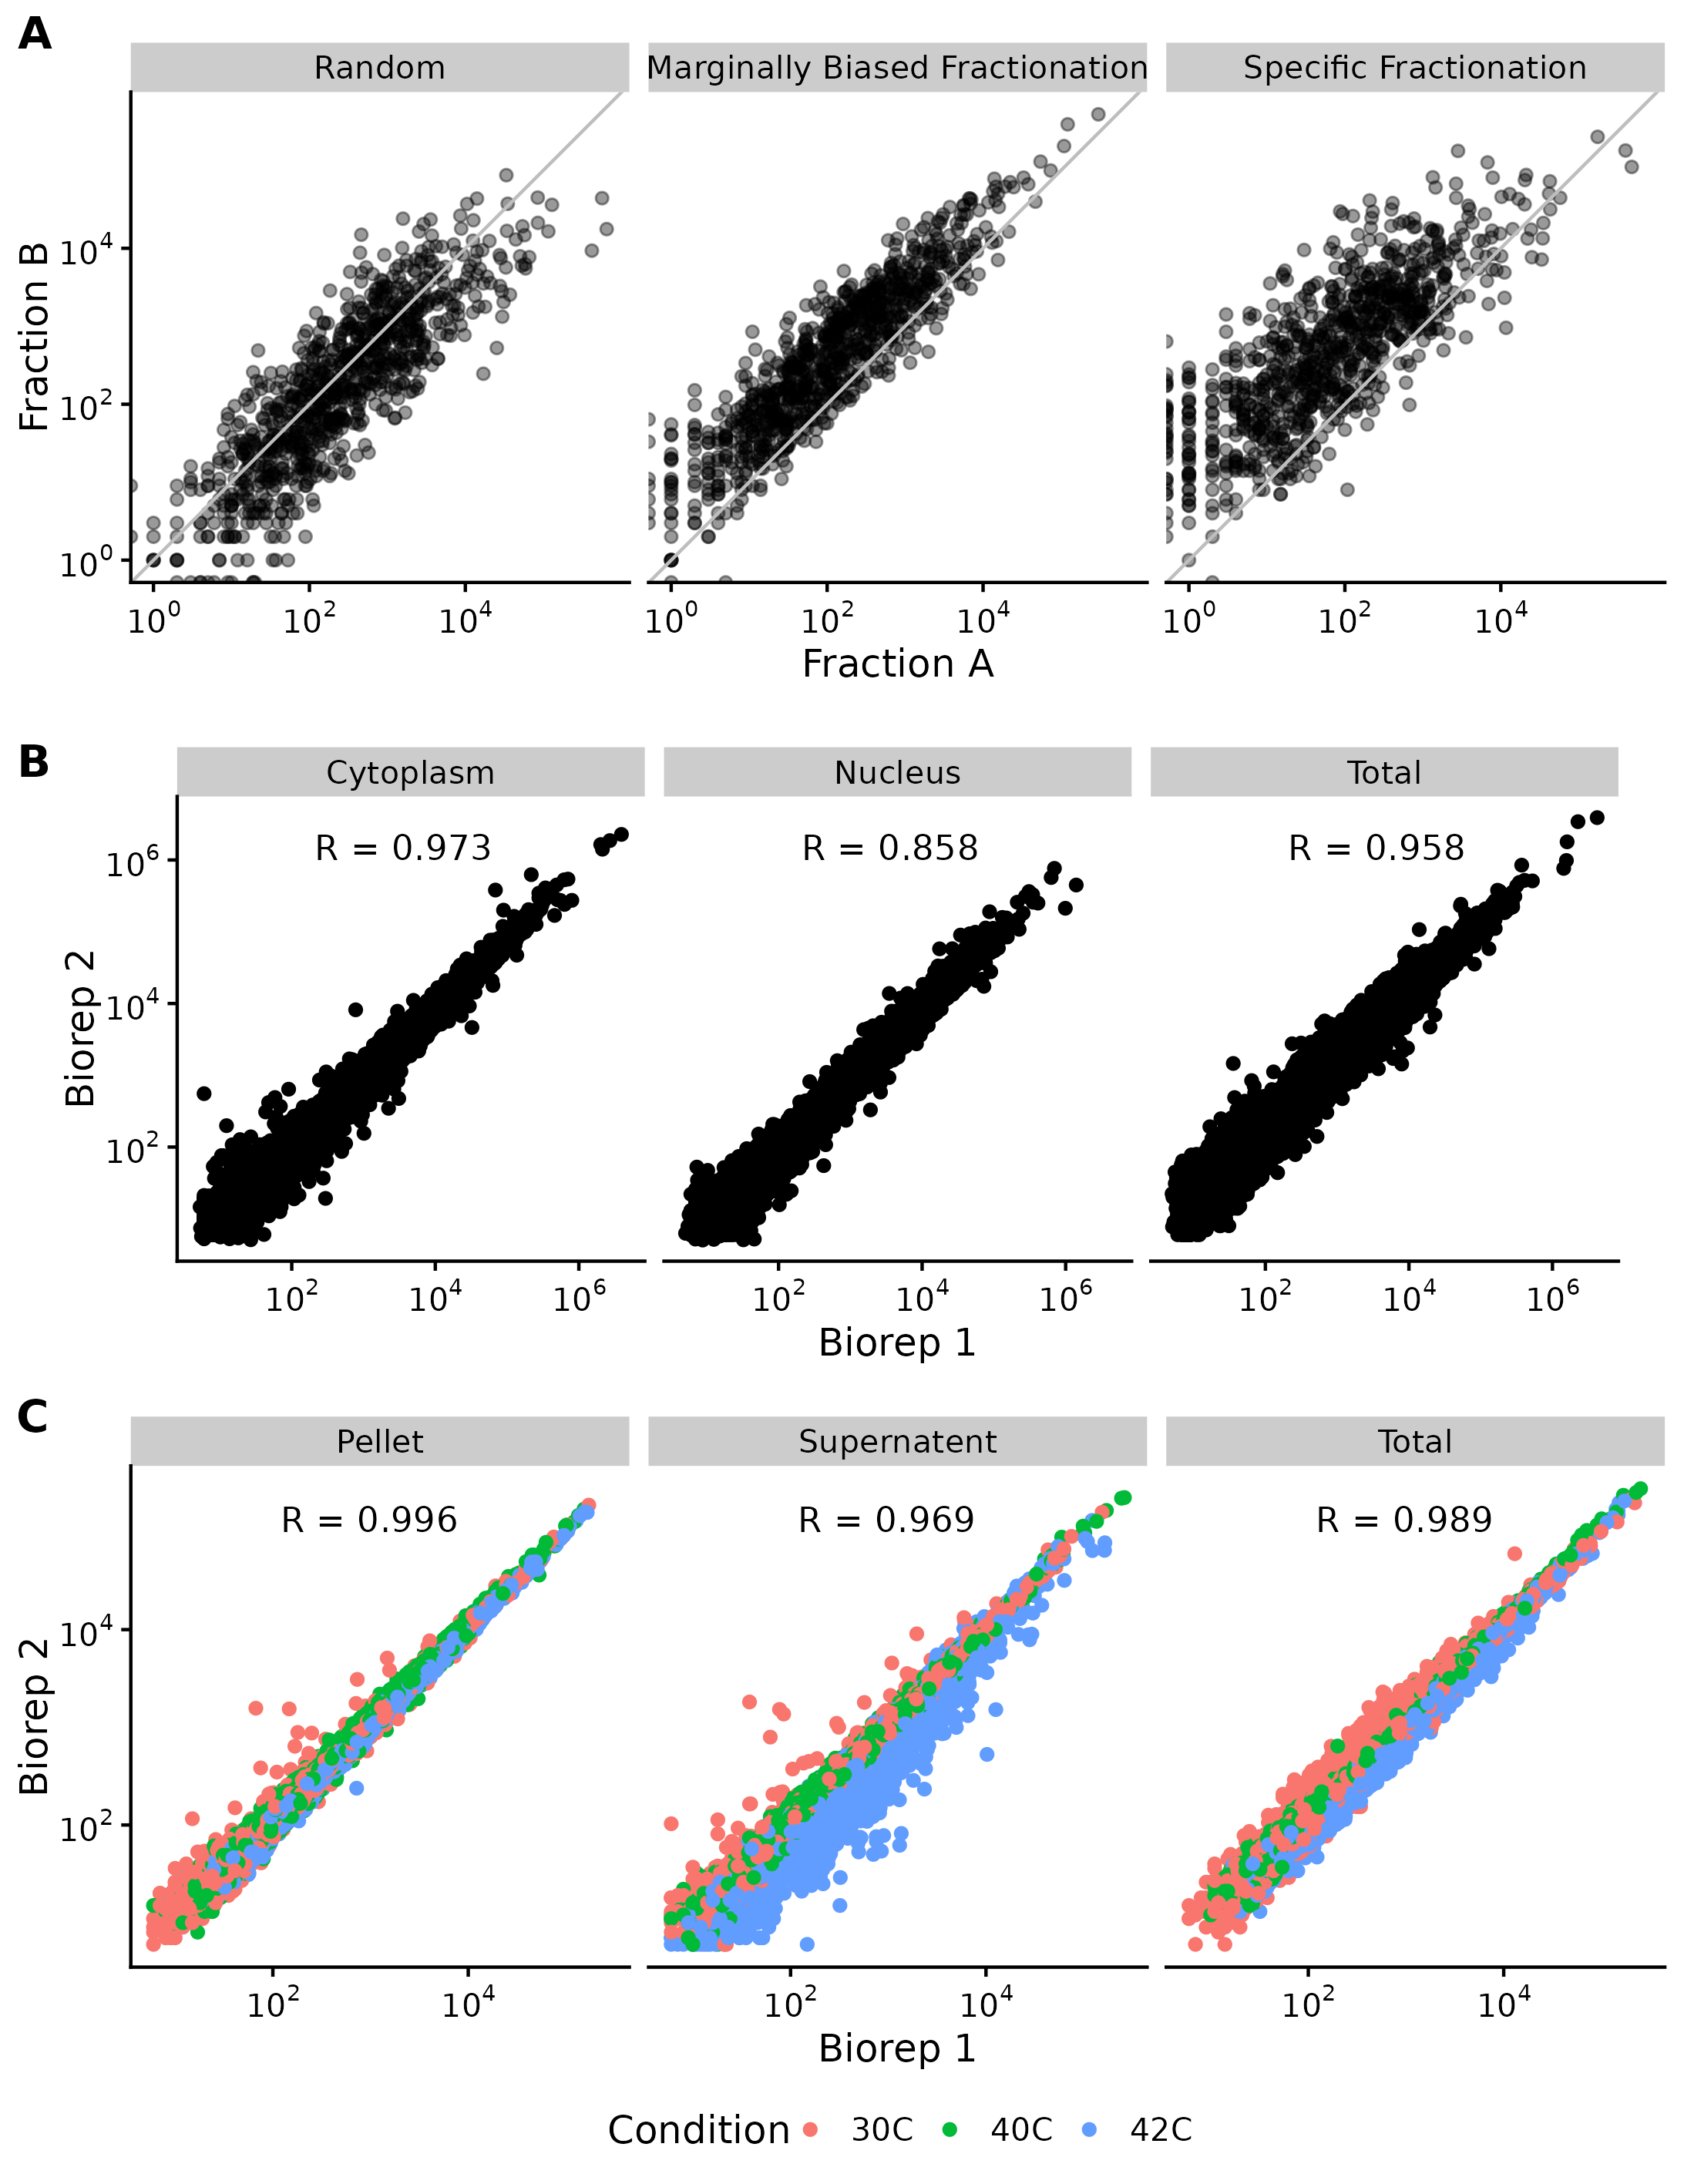
\includegraphics[width=0.8\linewidth]{figures/fractionation_dataset_summary.png} 

}

\caption[Overview of fractionation data sets.]{\textbf{Overview of the two experimental and one simulated data sets used in this study.} \textbf{(A)}  Simulated mRNA transcript counts between two fractions in three regimes: all gene are randomly allocated a fraction, most genes have a marginal bias towards fraction B, and the majority of transcripts are in fraction B but transcripts from a specific subset of genes are found in fraction A. 
\textbf{(B)} Correlation between two biological replicates of nuclear vs cytoplasmic mRNA transcript counts in a human lymphoblastoid cell line from the ENCODE project \parencite{Dunham2012}. \textbf{(C)} Correlation between two biological replicates of mRNA transcript counts in heat shock induced stress granules vs freely floating in \textit{Saccharomyces} cerevisiae cells. The dataset includes three temperature conditions: optimal 30C, mild 40C heat shock, and extreme 42C heat shock  \parencite{Iserman2020}.} \label{fig:fractionation-datasets}
\end{figure}

\subsection{Quantifying Fractionation in the Simulated Data Set}

The three replicates of noisy $N^{Tot}$, $N^{A}$ and $N^{B}$ counts from each regime of the simulated data set are used to train the DiffFracQuant model.
1000 samples of $\lambda^{A}$ and $\lambda^{B}$ are taken from the posterior distribution after a 1000 iteration burn-in.
A gene is considered to be significantly localised to fraction B if 97.5\% of the $\lambda^{B}$ samples are greater than $\lambda^{A}$ for that gene in that regime.
DiffFracQuant is compared to the results from DESeq2 trained on $N^{A}$ and $N^{B}$ counts.
DESeq2 is used according to the standard workflow outlined in its documentation.
The workflow includes the determination of normalisation factors, estimation of dispersion and calculation of significance using a Wald test. 

The log$_2$ ratio of transcript counts between the two fractions as calculated by DESeq2 and DiffFracQuant were compared to the log$_2$ ratio of noiseless counts in the simulated data set, $\gamma/(1-\gamma)$, Figure \ref{fig:simulated-data-results}A.
The correlation between predicted log$_2$ ratio and ground truth is greater than 0.98 for both methods in all regimes. 
However, the disparity between the models develops as the ratio of transcript between fractions for each gene changes from a random distribution to being predominately localised in fraction A. 
The log$_2$ ratios from DiffFracQuant consistently match the ground truth across all conditions and magnitudes.
The log$_2$ ratios from DESeq2 shift down below the ground truth as the normalisation factors between fractions diverge because they begin to include some of the global changes in the transcriptome, Figure \ref{fig:simulated-data-results}B.
This behaviour is reflected in the detection of significant difference in transcript abundance between the two fractions.
Across all genes, DESeq2 has a larger false discovery rate (FDR) in the marginal and specific regimes than DiffFracQuant.
Although DESeq2 does have a marginally better FDR in the random regime its true positive rate (TPR) is notably less than DiffFracQuant, Figure \ref{fig:simulated-data-results}C.
This behaviour is replicated over the 60 least abundant genes and the 60 genes with the smallest change between the conditions, Figure \ref{fig:simulated-data-results}D.

\begin{figure}[p!]

{\centering 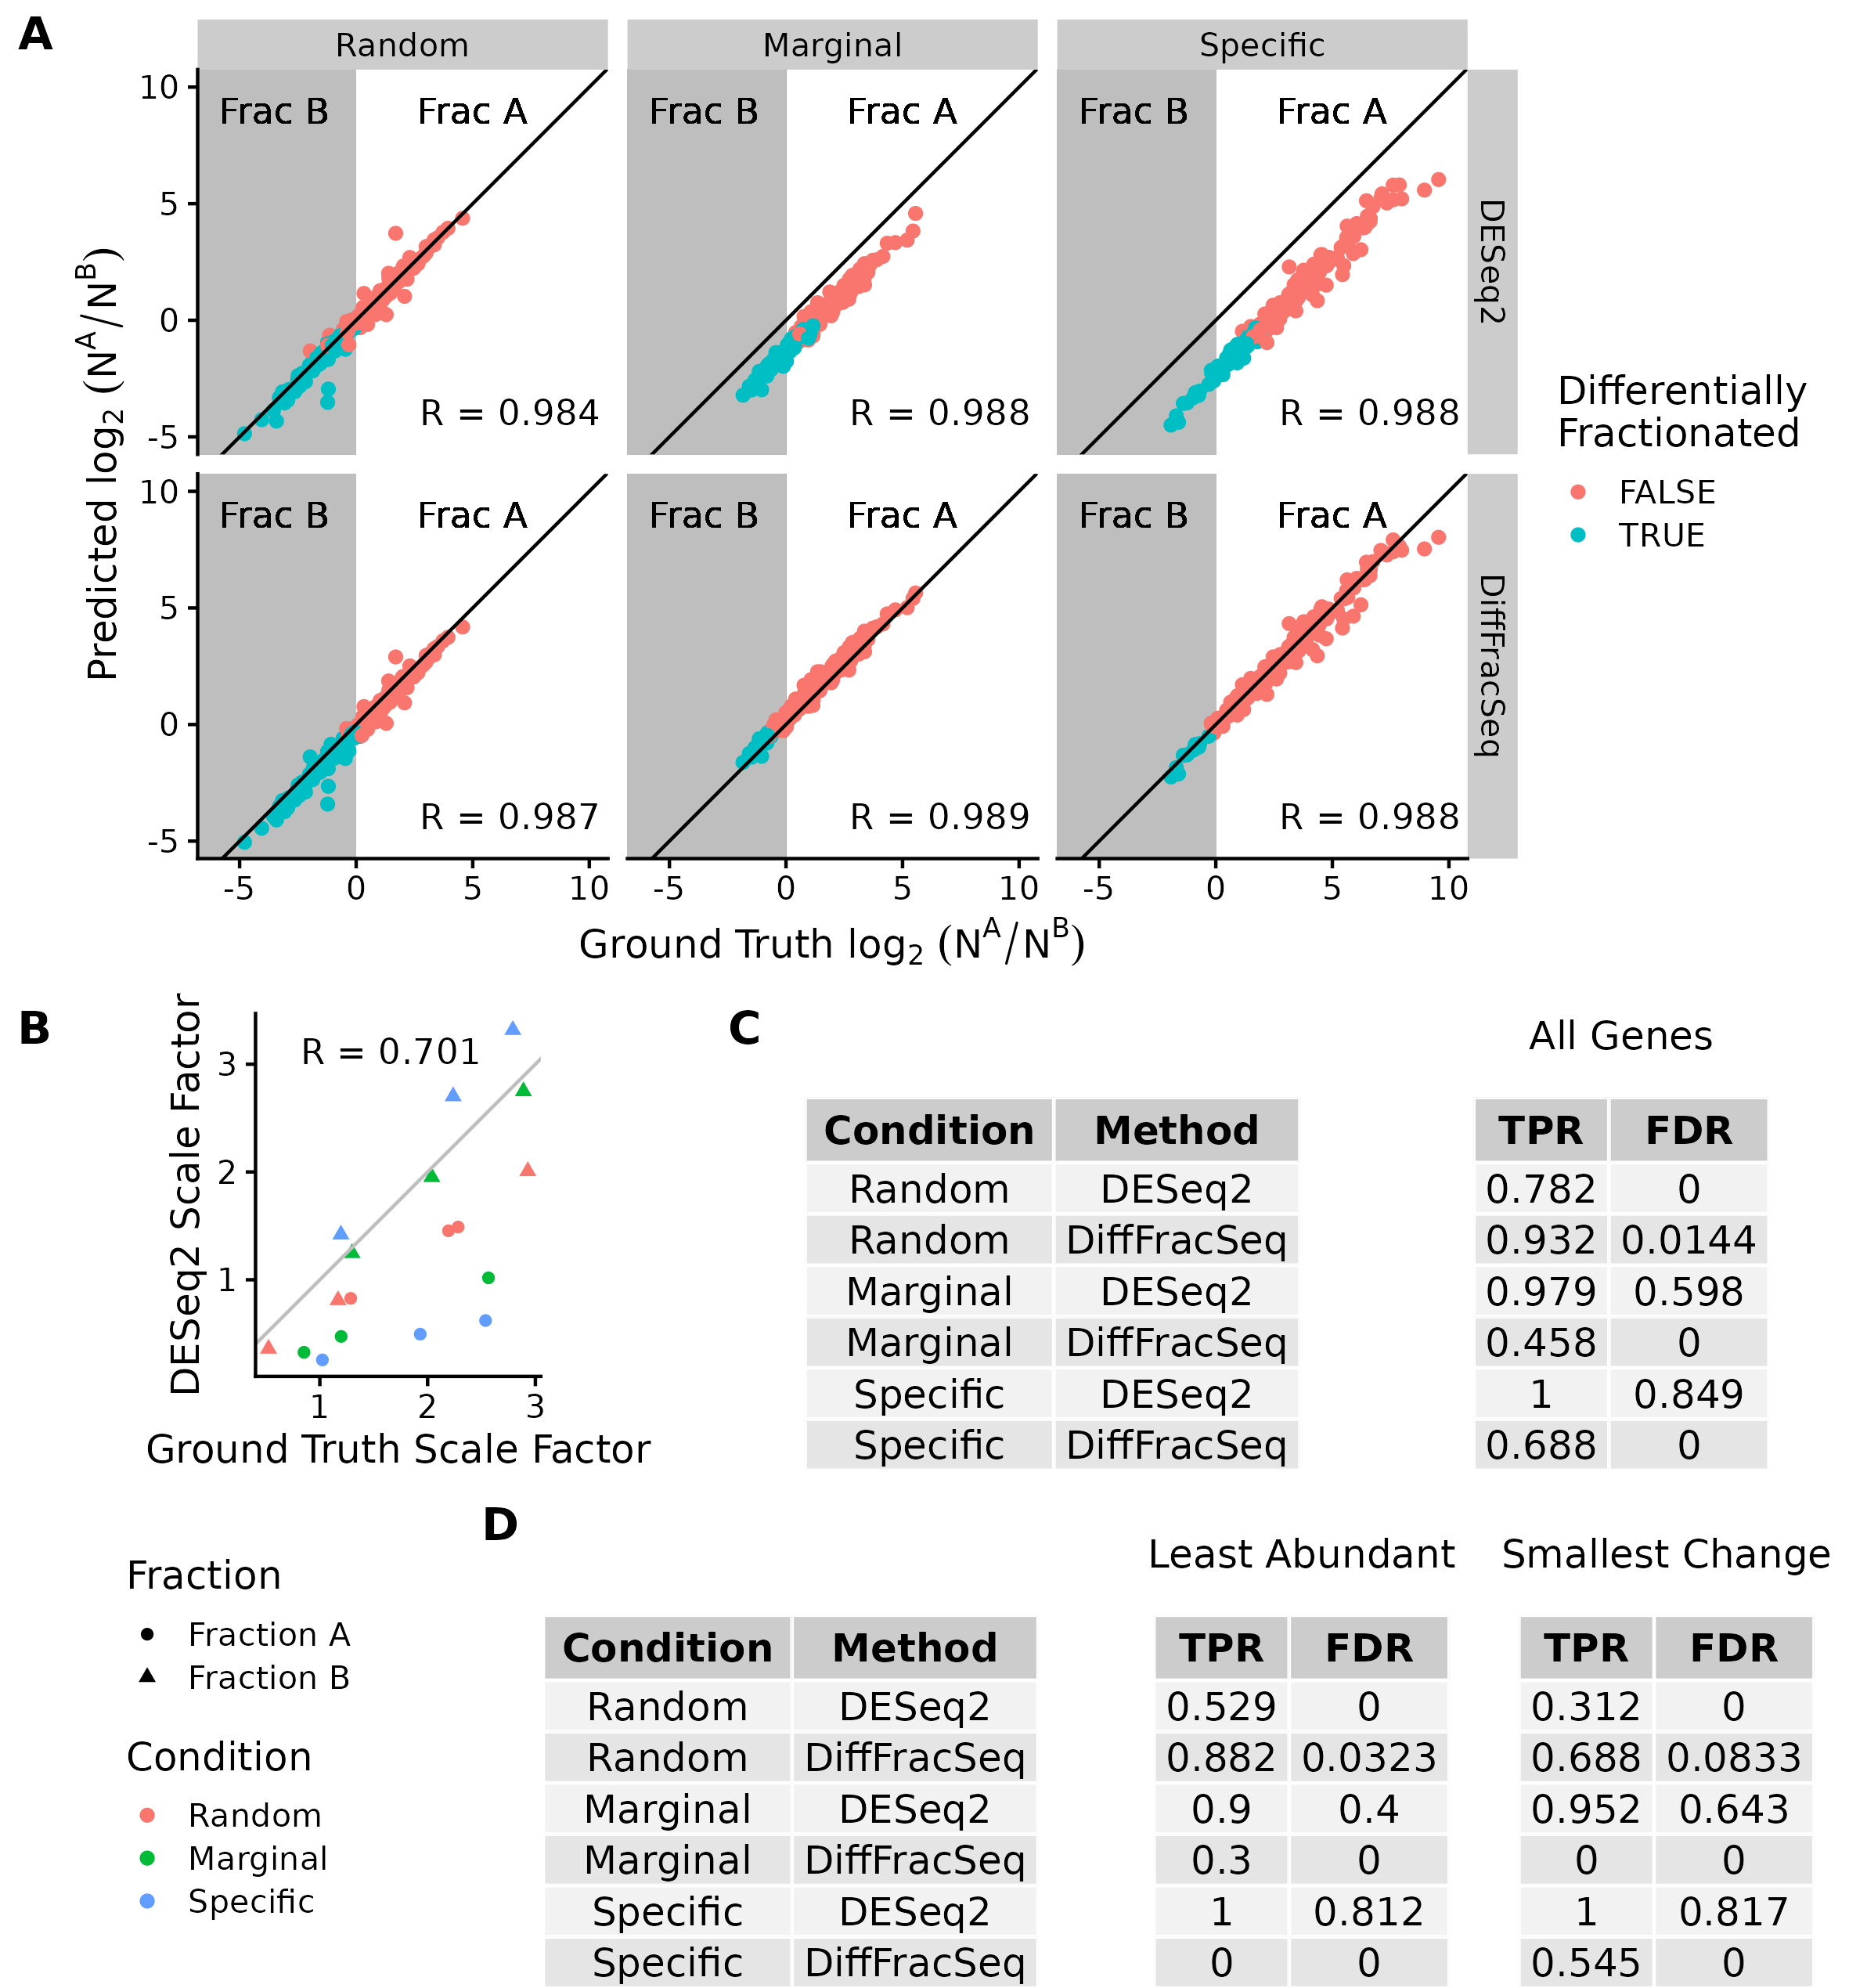
\includegraphics[width=1\linewidth]{figures/DESeq_vs_bayesian_combined.png} 

}

\caption[Simulated data performance.]{\textbf{Comparison of DESeq2 and DiffFracQuant performance a simulated data set.} \textbf{A} Predicted vs ground truth log$_2$ ratio of transcripts in fraction A to fraction B. The first row presents the results determined DESeq2 and the second row presents the results from DiffFracQuant. The results from the three regimes in the simulated data set are shown across the columns. \textbf{B} Comparison of DESeq2 values of RNA-Seq run specific total read scale factors to the ground truth. \textbf{C} True positive rates (TPR) and false discovery rates (FDR) of the two methods across three regimes for all genes. \textbf{D} Similar to \textbf{C} but across the 60 least abundance genes and the 60 genes with the smallest change between fractions.} \label{fig:simulated-data-results}
\end{figure}

\subsection{Quantifying Fractionation in the Experimental Data Sets}

The performance of DiffFracQuant compared to DESeq2 was next checked using the ENCODE nuclear vs cytoplasmic fraction data set. 
Similar to the results from the simulated data set, the correlation in log$_2$ fraction ratios between the two methods is high, but only DiffFracQuant is able to suggest an asymmetric distribution in total transcript counts between the two fractions, \ref{fig:encode-iserman-data-results}A.
DiffFracQuant determines that the majority of poly(A) tailed RNA transcripts are found in the cytoplasm as expected in an unstressed sample of cells grown in standard conditions.
Over half of the 234 genes that DiffFracQuant detects as having transcripts localised to the nucleus are associated with roles other than protein coding, according to the PANTHER database. 
These genes are also detected to be differentially fractionated by DESeq2 alongside 4708 others, 3471 of which are known to be protein coding.
The ENCODE data set was also used to investigate DiffFracQuant's ability to analysis data sets that do not contain any replicates. 
A case which is DESeq2 is unable to analysis.
The results between using one and two replicates are correlated, $R = 0.84$, but there are quite significant differences in the number of genes that are determined to be differentially expressed, especially in low abundant genes, \ref{fig:encode-iserman-data-results}B.

The Iserman \textit{et al} data set on stress granule formation over three temperatures enabled DiffFracQuant to be tested on a scenario similar to the simulated data set. 
DiffFracQuant and DESeq2 have similar correlations in log$_2$ ratio across the temperatures with a trend towards the same values as temperature increases.
The detection of differential fractionation diverges more between the methods in the Iserman \textit{et al} data set compared to the ENCODE data set.
A gene ontology analysis was conducted on genes detected to be differentially fractionated in the pellet at $40\degree$C by DiffFracQuant only and by DESeq2 only.
Although the DiffFracQuant only genes were not enriched with any particular ontological term the significant lack of transcripts relating to fundamental cell processes remains of note.
Meanwhile, the DESeq2 only genes included the expected number of genes relating to primary metabolic processes as well as being enriched with genes relating to transport. 

\begin{figure}[p!]

{\centering 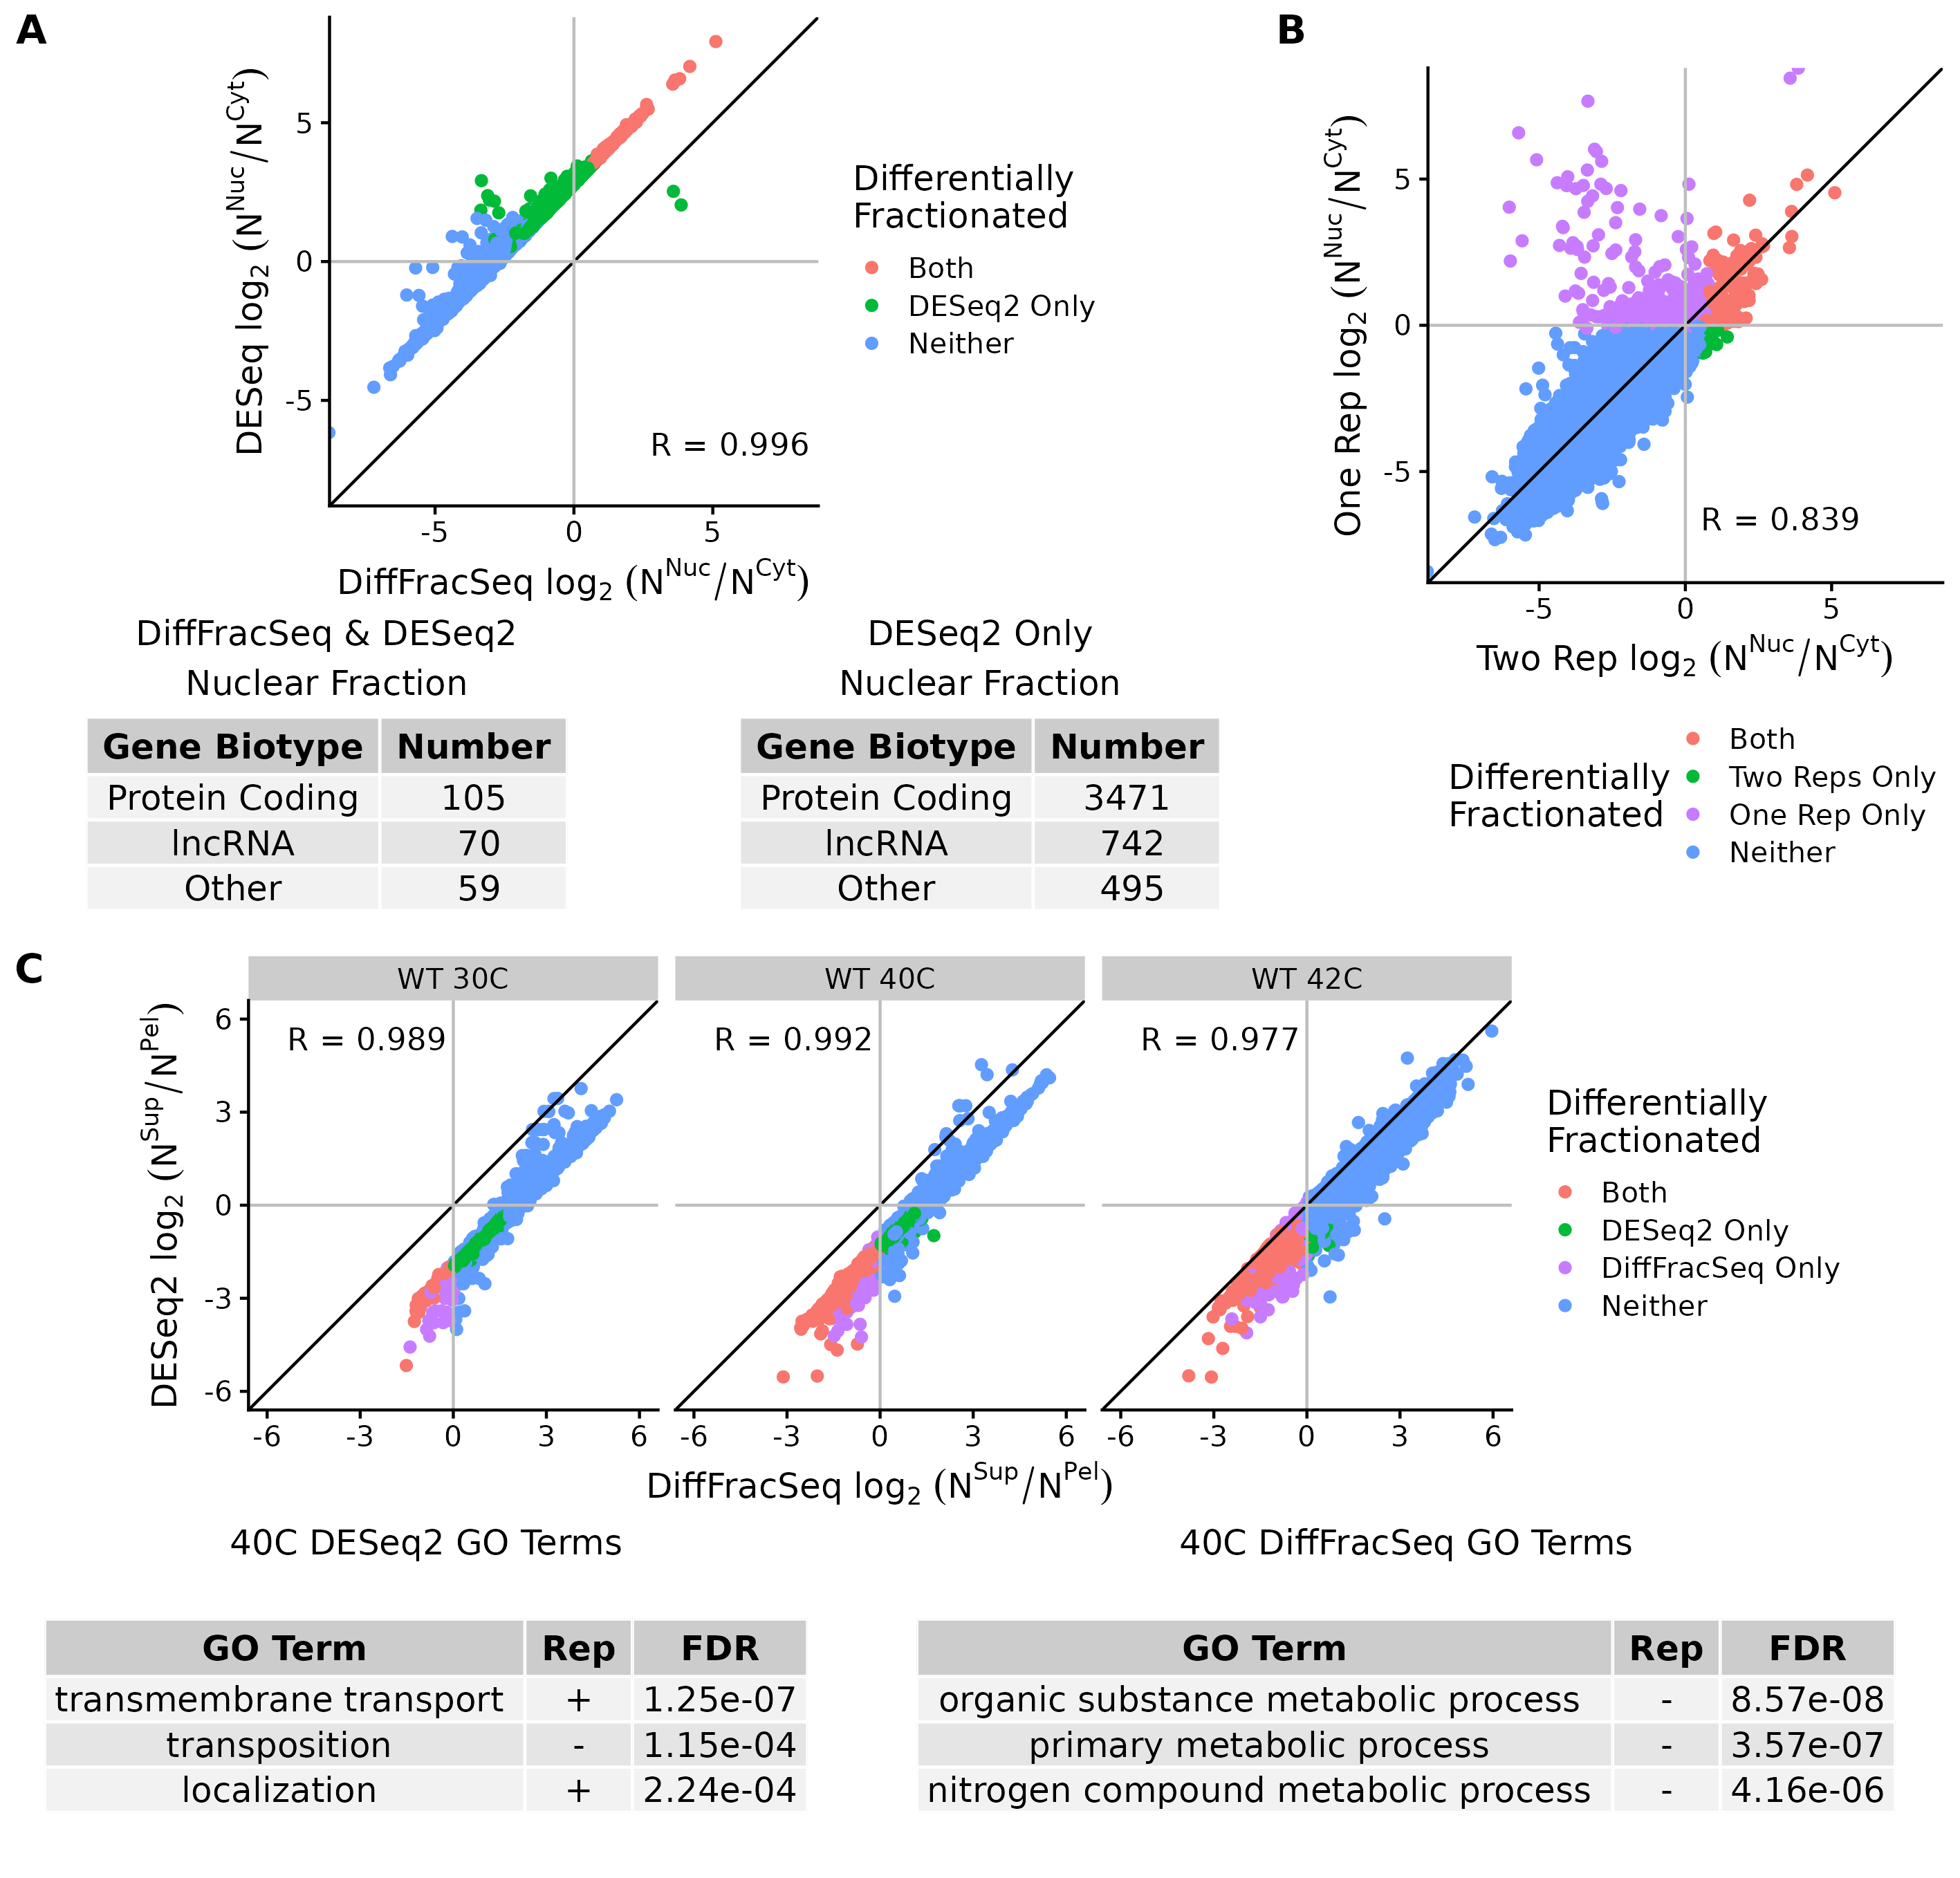
\includegraphics[width=1\linewidth]{figures/DESeq_vs_bayesian_encode_and_iserman_combined.png} 

}

\caption[Experimental data performance.]{\textbf{Comparison of DESeq2 and DiffFracQuant performace on two experimental data sets.} \textbf{(A)} DESeq2 vs DiffFracQuant predicted log$_2$ ratio of transcripts in the nucleus to the cytoplasm from the ENCODE data set. The two tables show the associated biotype of genes considered differentially fractionated either by both methods or by DESeq2 only, as retrieved from PANTHERdb. \textbf{(B)} DiffFracQuant predicted log$_2$ ratio of transcripts when trained with both or only one of the biological replicates in the ENCODE data set. \textbf{(C)} DESeq2 vs DiffFracQuant predicted log$_2$ ratio of transcripts in the supernatent to the pellet from the Iserman \textit{et al} data set. The wildtype samples across three temperature conditions are shown across the columns. The two tables show the top three terms in a gene ontology analysis conducted on genes that are considered differentially fractionated either by DESeq2 only or by DiffFracQuant only in the $40\degree$C condition. The second column of each table denotes whether the GO term is overrepresented ($+$) or underrepresented ($-$) in the gene group.} \label{fig:encode-iserman-data-results}
\end{figure}

\subsection{Detecting Changes in Fractionation and Total Expression Across Conditions}

The samples from three temperatures available in the Iserman \textit{et al} data set can be used to test DiffFracQuant's ability to detect changes in global expression as well as changes in fractionation. 
First, the predicted change in transcript in the same supernatent fraction across the temperatures is high correlated between DESeq2 and DiffFracQuant, Figure \ref{fig:diff-exp-temp}A. 
Combining DiffFracQuant's ability to detect changes in fractionation and in total expression , Figure \ref{fig:diff-exp-temp}B.
There is a clear correlation between gene predicted to have an increase in total expression and genes that change to be more concentrated in the supernatent.
The results display four distinct behaviours as temperature increases: genes that increase expression and fractionation into the pellet, genes that decrease expression and fractionation into the pellet,  genes that increase expression but decrease fractionation into the pellet, and genes that decrease expression but increase fractionation into the pellet.
There is a distinct shift between lower expression and higher pelleting as the temperature increases to 42$\degree$C.
There is less difference in pelleting and expression between the two stress temperatures compared to either tempertaure and 30$\degree$C.

\begin{figure}[p!]

{\centering 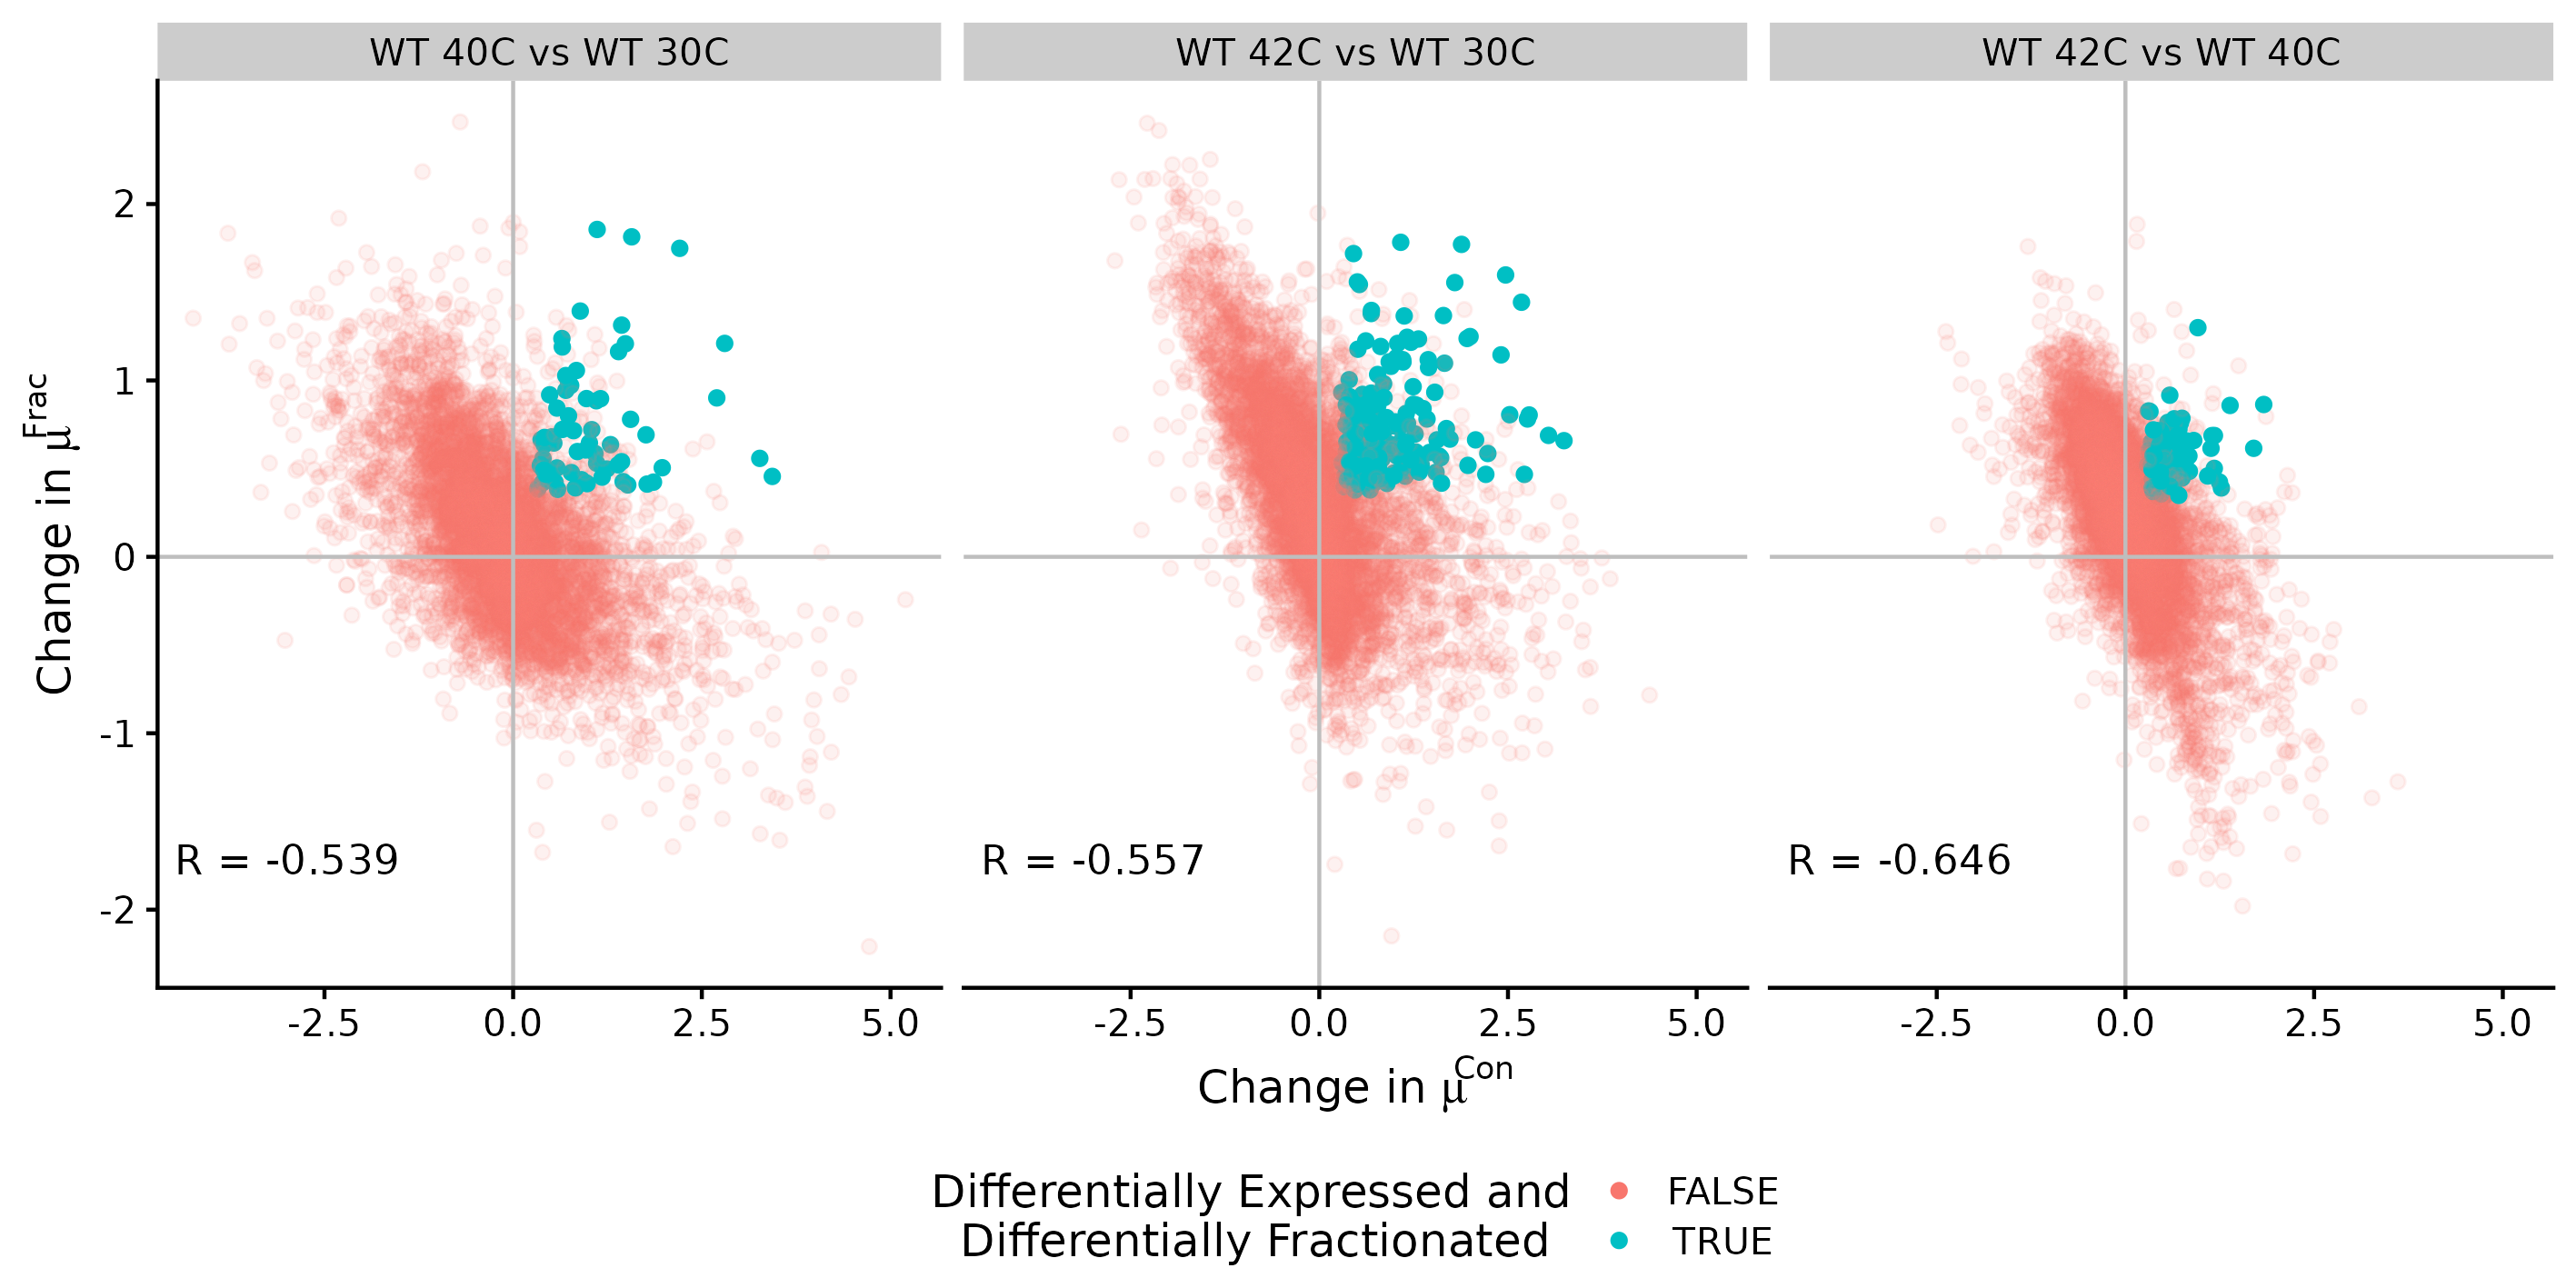
\includegraphics[width=1\linewidth]{figures/DESeq_vs_bayesian_multi_temp_iserman_combined.png} 

}

\caption[Differential fractionation across conditions.]{\textbf{Detection of differential fractionation and differential expression across the Iserman data set.} \textbf{(A)} Comparison of log2 fold change in the supernatent fraction across the three temperatures as detected by DESeq2 and DiffFracQuant. \textbf{(B)} Simultaneously investigating differential fractionation and differential expression across the three temperature conditions according to DiffFracQuant.} \label{fig:diff-exp-temp}
\end{figure}

\section{Chapter 5 Conclusion}

This chapter introduced DiffFracQuant as a novel Bayesian model for the detection of differential fractionation.
DiffFracQuant's is shown to outperform DESeq2 in detecting differential fractionation using a simulated data set, a human lymphoblastoid data set and a \textit{Saccharomyces} cerevisiae data set.
The model's ability to perform even with a single replicate data set and to extract changes in total transcript abundance as well as relative fractions from data sets with multiple conditions means it is versatile tool in exploring fractionation data sets.

The two methods performance at determining supernatent to pellet fractions using the Iserman \textit{et al} is notably comparable to that on the simulated data sets. 
This can be explained as at $30\degree$C pelleting would be expected to be quite specific as few, if any, stress granules should be present.
At $42\degree$C, broad pelleting would be expected as the highly stressed cells would undertake significant stress granule formation and random transcript allocation would increase. 
Meanwhile, the detection of differential expression in the same fraction across conditions is exactly what DESeq2 is designed to handle so DiffFracQuants comparable performance highlights its reliability.
Finally, combining the total expression changes and differential fractionation with DiffFracQuant offers insight into the complex way cells can change their entire transcriptomes in response to stress.

The software is available to download from GitHub and has been shown to be successful at investigating localisation across organisms and subcelluar fractions.
Alternatively, this software could be used to characterise libraries of constructs by comparing fractions from cell sorting assays.
Entire libraries of synthetic constructs can be characterised by sorting pools of constructs by some desired characteristic, for example high protein fluorescence, which are subsequently sequenced \parencite{Sharon2012}. 
DiffFracQuant has the functionality to improve the quality of experiments across biology from the uncovering of novel regulatory mechanisms in fundamental cell biology to the characterisation of constructs libraries in synthetic biology.

\end{document}